\documentclass[floatsintext, man]{apa7}
\usepackage[style=apa, backend=biber]{biblatex}
\addbibresource{lit.bib}
\usepackage[justification=centering]{caption}
\usepackage{amsmath}
\usepackage{amssymb}
\usepackage{enumerate}

\title{Bayesian Psychometrics}
\shorttitle{Bayesian Psychometrics}
\journal{International Encyclopedia of Education}

\authorsnames{Xiang Liu, Matthew S. Johnson, Zhuangzhuang Han}
\authorsaffiliations{Educational Testing Service}
\keywords{Bayesian, psychometrics, IRT, MCMC, posterior predictive model checks}
\abstract{The application of Bayesian methods in psychometrics is getting
popular. It offers a set powerful and flexible statistical tools for analyzing
psychometric data. In this entry, we provide a brief introduction of essential
concepts of Bayesian data analysis - model formulation, posterior computation,
and model fit evaluation. These concepts are demonstrated by using a simple
1-parameter normal ogive IRT model as an example.}

\begin{document}
\maketitle
\section{Introduction}
Bayesian statistical methods have become popular in the field of psychometrics.
Thanks to the development of general purpose Bayesian inference software (e.g.,
\emph{Stan}; \cite{gelman_stan:_2015}), researchers are now able to quickly develop and
fit sophisticated and complex psychometric models that once required significant
computational expertise to estimate. \textcite{levy_rise_2009} gives a nice overview
and survey of the applications of Bayesian estimation for psychometric models.
Some examples of development in this area may include Bayesian estimation of a
broad class of cognitive diagnostic models 
\parencite{liu_estimating_2019,culpepper_bayesian_2015}, the
extended marginal Rasch model \parencite{maris_gibbs_2015}, a multilevel item
response theory (IRT) model \parencite{fox_bayesian_2001}, and an unfolding
response model \parencite{johnson_using_2003}. In addition, Bayesian
methods also provide a class of approaches alternative to classical or
frequentist statistics (e.g. maximum likelihood, confidence intervals,
p-values). In certain cases, Bayesian approaches can alleviate some difficulties
classical approaches may have. Examples of the use of Bayesian methods for psychometric modeling include estimating uncertain elements of the Q-matrix in a CDM
model \parencite{decarlo_recognizing_2012}, nonparametric ordered latent class
modeling \parencite{liu_three_2019}, robust IRT outlier detection 
\parencite{ozturk_bayesian_2017}, and evaluating model fit 
\parencite{sinharay_assessing_2007,sinharay_assessing_2005,sinharay_assessment_2015}. These mentioned examples of Bayesian methods in psychometrics are far from exhaustive.
The main purpose of this entry is to give readers a brief introduction to some
of the most essential concepts and steps involved in a Bayesian analysis of
psychometric models.

\section{Bayesian data analysis}
Let $\bm{X}$ denote the observed random variables (i.e. the data), and $
\bm{\theta}$ denote the vector of unobserved random variables (i.e. the
parameters). In Bayesian statistics, the parameters are treated as random and
are given prior distributions. This is in contrast to the classical likelihood
methods where parameters are treated as fixed but unknown parameters. We are
typically interested in using the data to estimate and make inferences about the
vector of unknown parameters. A Bayesian analysis involves three essential
steps:
\begin{enumerate}
  \item Model specification. In this step, we set up a full probability model
  that describes the joint probability distribution for all observed and
  unobserved random variables, i.e. $p(\bm{X}, \bm{\theta})$. According to the
  definition of conditional probability, this joint probability distribution can
  be factorized as $p(\bm{X}, \bm{\theta}) = p(\bm{X}|\bm{\theta})p(
  \bm{\theta})$. The marginal density, $p(\bm{\theta})$, is often referred to as
  the \textit{prior distribution} which expresses any prior belief we may have
  on the parameters with uncertainty, and the conditional density, $p(\bm{X}|
  \bm{\theta})$, is called the \textit{sampling distribution} (or the generating
  distribution) which describes the data generation process. Setting up these
  models generally requires some knowledge of the underlying problems with,
  sometimes, considerations for mathematical convenience.

  \item Posterior inference. In this step, we calculate and interpret the
  \textit{posterior distribution} from which we make inferences about the
  parameters. The posterior distribution is the conditional
  distribution of the unobserved random variables (i.e. parameters) which we are
  typically interested in, given the observed data, i.e. $p(\bm{\theta}|\bm{X})
  = p(\bm{\theta}, \bm{X}) / p(\bm{X}) = p(\bm{X}|\bm{\theta})p(\bm{\theta}) /
  p(\bm{X})$. This is known as Bayes' rule. As a function of parameters $
  \bm{\theta}$, $p(\bm{X}|\bm{\theta})$ is also referred to as the likelihood
  function through which the data $\bm{X}$ influences the posterior distribution
  of the parameters. To obtain the density of the marginal distribution of the
  data, we need to evaluate $p(\bm{X}) = \int p(\bm{X}|\bm{\theta})p(
  \bm{\theta}) d\bm{\theta}$. Except for certain extremely simple models, this 
  (potentially high dimensional) integral cannot be evaluated analytically.
  Consequently, the posterior is generally not available in closed forms.
  Instead, the posterior distribution $p(\bm{\theta}|\bm{X})$ is usually
  approximated using sampling methods such as the Markov chain Monte Carlo 
  (MCMC; \cite{neal_probabilistic_1998,gelman_bayesian_2013}).

  \item Model fit evaluation. Once a model has been set up and the posterior
  distribution has been computed, it is important to assess the fit of the
  model. Inferences drawn from a model that does not fit well could be very
  misleading. In a Bayesian framework, the assessment of model fit is typically
  performed through the posterior predictive model checking (PPMC; 
  \cite{gelman_bayesian_2013,rubin_bayesianly_1984}). If the model fits
  reasonably well, the observed data or
  the derived statistics of our practical interest should look plausible under
  the posterior predictive distribution. The identified aspects of model misfit
  could help improve or expand the model. Sometimes, identifying misfit itself
  could be of practical interest, for example, to identify aberrant response
  patterns (e.g. \cite{sinharay_assessment_2015}).
\end{enumerate}

These steps are applicable to Bayesian modeling for all applications. Bayesian
psychometrics is the application of these steps to psychometric modeling.
In the following sections, we demonstrate these essential steps of the Bayesian
data analysis with a little more details by using a simple 1-parameter normal
ogive IRT model as an example.

\section{Model specification} 
Let $X_{ij} = x_{ij}$ be a dichotomous random variable of the item response from
the $i^{th}$ student to the $j^{th}$ item, $i = 1, 2, \dots, N$ and $j = 1, 2,
\dots, J$. And $x_{ij} = 1$ if the response is correct, $x_{ij} = 0$ otherwise.
Under the 1-parameter normal ogive (1PNO) IRT model, the probability of a
correct response is given by 
\begin{equation}
\label{eq:1PNO_with_a}
  P(X_{ij} = 1 | \theta_i, a, b_j) = \Phi(a(\theta_i - b_j)),
\end{equation}
where $\Phi(\cdot)$ denotes the cumulative probability density function (CDF) of
the standard normal distribution, $\theta_i$ is the person parameter, $b_j$ is
the item difficulty parameter, and $a$ is the common discrimination parameter
shared among $J$ items. The person parameter is assumed to follow a standard
normal distribution, i.e. $\theta_i \sim N(0,1)$. Because $a$ is a constant
across items, the item characteristic curves (ICC) never cross each other and
only differ by locations (see Figure~\ref{fig:ICC}).
\begin{figure}[t]
\centering
  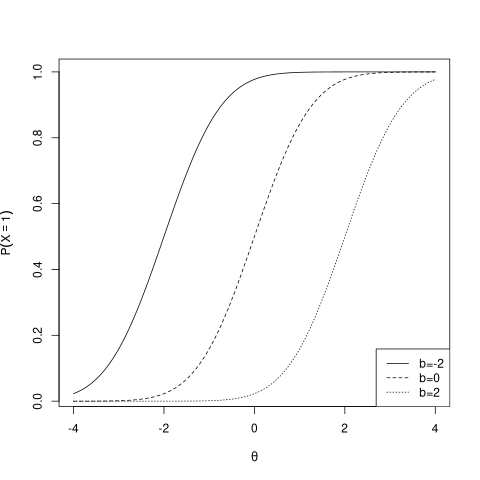
\includegraphics[scale=0.5]{Fig/ICC.png}
  \caption{ICC of the 1PNO IRT model}
  \label{fig:ICC}
\end{figure}

The 1PNO as in Equation~\ref{eq:1PNO_with_a} can be expressed as a Bayesian
hierarchical model. For computational efficiency, we reparameterize the model so
that the model is in its slope-intercept form,
\begin{equation}
  \label{eq:1PNO}
  P(X_{ij} = 1 | \theta_i, \psi_j) = \Phi(\theta_i + \psi_j),
\end{equation}
and $\theta_i \sim N(0, a^2)$, where $a^2$ is the variance of the normal
distribution.

A prior distribution describes any prior belief we may have (or the lack of it)
on the parameter with uncertainty. For instance, in the current example, there
may be reasonable prior information on the item parameter $\psi_j$ from similar
items previously administered to a
comparable population of students. In this case, we may choose a normal prior
with mean $\mu_{\psi_j}$ informed by prior information and variance $\sigma_
{\psi_j}^2$ expressing the level of
uncertainty, i.e. $\psi_j \sim N(\mu_{\psi_j}, \sigma_{\psi_j}^2)$. A prior with
larger variance (or a flatter prior, see Figure~\ref{fig:prior_density}) is
less informative and appropriate when there is greater uncertainty about a
parameter, thus having less impact on the posterior inference of the parameter. 
\begin{figure}[t]
\centering
  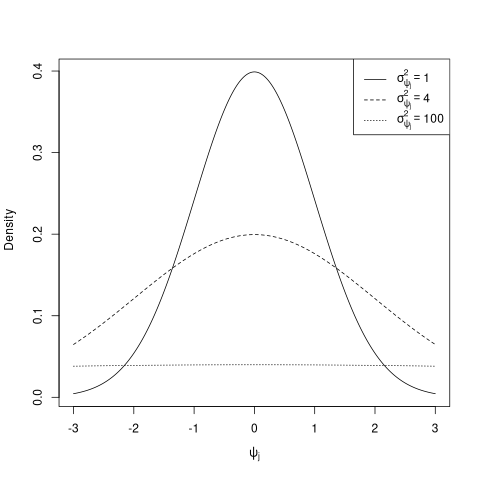
\includegraphics[scale = 0.5]{Fig/prior_normal.png}
  \caption{Density of prior distribution of $\psi_j$}
  \label{fig:prior_density}
\end{figure}
However, prior information may not always be available. In this case, instead of
choosing a fixed prior with a large variance, an alternative approach is to use
a hierarchical prior. For each item parameter $\psi_j$, we assign a same
Gaussian prior, $\psi_j \sim N(\mu_\psi, \sigma_\psi^2)$. Hyper-priors are
assigned to the parameters of this prior distribution, i.e. $\mu_\psi \sim N(0,
10^2)$ and $\sigma_\psi^2 \sim Ga^{-1}(10^{-4}, 10^{-4})$, where $Ga^{-1}
(\cdot)$ denotes the inverse-gamma distribution (see 
\cite{gelman_bayesian_2013}, p.43). The chosen inverse-gamma distribution is
noninformative if most of the posterior density is away from $0$
as the prior density is flat in the tail. The choice of this set of priors is
also mathematically convenient. The normal prior and inverse-gamma prior are
conditionally conjugate for the model. A prior is said to be conjugate for the
likelihood function if the resulting posterior distribution is in the same
probability distribution family. In this case, the conditional posteriors for
the mean parameter and the variance parameter normal and inverse-gamma. We
choose a similar noninformative inverse-gamma distribution for
$a^2$, i.e. $a^2 \sim Ga^{-1} (10^{-4}, 10^{-4})$. We can then write the 1PNO
IRT model has a Bayesian hierarchical model,
\begin{equation}
\label{eq:1pno_original}
\begin{gathered}
  x_{ij} | \theta_i, \psi_j \sim Bernoulli(\Phi(\theta_i + \psi_j))\\
  \psi_j | \mu_\psi, \sigma_\psi^2 \sim N(\mu_\psi, \sigma_\psi^2)\\
  \mu_\psi \sim N(0, 10^2)\\
  \sigma_\psi^2 \sim Ga^{-1}(10^{-4}, 10^{-4})\\
  \theta_i | a^2 \sim N(0, a^2)\\
  a^2 \sim Ga^{-1}(10^{-4}, 10^{-4}).
\end{gathered}
\end{equation}

\section{Posterior inference}
For any practical applications, we are interested in inferring model parameters
given the data, in other words, computing the posterior distribution. The
\textit{joint} posterior distribution of the parameters, $p(\bm{\theta}, 
\bm{\psi}, \mu_\psi, \sigma_\psi^2, a^2 | \bm{x})$, cannot be analytically
computed. As a result, we use MCMC to sample from this unknown distribution. The
simplest MCMC algorithm is perhaps the Gibbs sampling. A Gibbs sampler
\parencite{geman_stochastic_1984} works by iteratively sampling from the full
conditional distributions of the parameters. Generally, this is feasible if the
full conditional distributions can be computed in closed form and sampled from
easily. However, this may not be true for some models. In these cases, other
MCMC algorithms are required, e.g. the Metropolis-Hastings algorithm 
\parencite{hastings_monte_1970}. The literature on MCMC algorithms is vast, and
the development of new MCMC methods is still an extremely active research area.
Readers may refer to \textcite{gelman_bayesian_2013,neal_probabilistic_1998} for
some detailed introduction and review on this topic.

For our example of the 1PNO model, a direct Gibbs sampling is possible. However,
we would need to augment latent variables. For every item response $x_{ij}$,
there is a latent variable $y_{ij}$ associated. The relationship between them is
deterministic such that
\[ x_{ij} = \begin{cases} 
            1 \text{ if } y_{ij} > 0,\\
            0 \text{ otherwise},
            \end{cases}
\]
where $y_{ij} \sim N(\theta_i + \psi_j, 1)$. It is straightforward to verify
that, under this specification, the probability of a correct response remains
$\int_{-\infty}^{\theta_i + \psi_j} \phi(y) dy = \Phi(\theta_i + \psi_j)$.

To derive the densities full conditional distributions, we use the definition of
conditional probabilities and the chain rule. For example,
\begin{equation}
\label{eq:full conditional y}
  p(y_{ij}|x_{ij}, \theta_i, \psi_j) = \frac{p(x_{ij}|y_{ij})p(y_{ij}|\theta_i,
  \psi_j)}{\sum_{y_{ij}}p(x_{ij}|y_{ij})p(y_{ij}|\theta_i, \psi_j)}.
\end{equation}
Notice that the denominator of Equation~\ref{eq:full conditional y} is a
constant (with respect to $y_{ij}$) that normalizes the full conditional
density. Therefore, we can conveniently write
\begin{align*}
  p(y_{ij}|x_{ij}, \theta_i, \psi_j) &= C p(x_{ij}|y_{ij})p(y_
  {ij}|\theta_i, \psi_j)\\
  & \propto p(x_{ij}|y_{ij})p(y_{ij}|\theta_i, \psi_j).
\end{align*}
Given that $p(x_{ij}|y_{ij})$ is a piecewise point density with support on
either $x_{ij} = 1$ or $x_{ij} = 0$ depending on $y_{ij}$, the full conditional
distribution of $y_{ij}$ is a truncated normal distribution, i.e.
\[
  y_{ij}|x_{ij},\theta_i,\psi_j \sim \begin{cases}
  &N(\theta_i + \psi_j, 1)T(0,) \text{ if } x_{ij} = 1,\\
  &N(\theta_i + \psi_j, 1)T(,0) \text{ if } x_{ij} = 0.
  \end{cases}
\]
$T(0,)$ denotes that the distribution is truncated with a lower bound of 0;
while $T(,0)$ denotes a truncation with a upper bound of 0.

The full conditional distributions of other parameters can be derived similarly.
Since the priors are chosen so that they are \textit{conditionally} conjugate,
the full conditional distributions of the parameters are within the same
distribution families as their priors. The standard conjugacy results apply (for
a reference, see \cite{gelman_bayesian_2013}). Here, we state the results without
detailed derivations.

Now we can summarize the Gibbs sampler. After assigning initial values to
parameters, at the $T^{th}$ iteration,
\begin{enumerate}
  \item for each $i$ and $j$, update $y_{ij}$ by drawing from $N(\theta_i +
  \psi_j, 1)T(0,)$ if $x_{ij} = 1$; else draw from $N(\theta_i + \psi_j, 1)T
  (,0)$;
  \item for each $i$, update $\theta_i$ by drawing from $N\left(\frac{1}{1/a^2 +
  J}(\sum_j (y_{ij} - \psi_j)), (1/a^2 + J)^{-1}\right)$;
  \item for each $j$, update $\psi_j$ by drawing from $N\left(\frac{1}
  {1/\sigma_\psi^2 + N}(\mu_\psi / \sigma_\psi^2 + \sum_i(y_{ij} -
  \theta_i)), \frac{1}{1/\sigma_\psi^2 + N}\right)$;
  \item update $a^2$ by drawing from $Ga^{-1}(10^{-4} + \frac{N}{2}, 10^{-4} +
  \frac{\sum_i \theta_i^2}{2})$;
  \item update $\mu_\psi$ by drawing from $N\left(\frac{1}{1/10^2 +
  J/\sigma_\psi^2}(\frac{\sum_j \psi_j}{\sigma_\psi^2}), (1 / 10^2 + J /
  \sigma_\psi^2)^{-1}\right)$;
  \item update $\sigma_\psi^2$ by drawing from $Ga^{-1}\left(10^{-4} + J
  / 2, 10^{-4} + \frac{\sum_j (\psi_j -\mu_\psi)^2}{2}\right)$.
\end{enumerate}
Keep updating long enough, the draws are eventually random samples from the
joint posterior distribution. Even though the theory of Markov chains guarantees
the eventual convergence to the desired target distribution which is the joint
posterior (see \cite{neal_probabilistic_1998}, for a review), in practice, we
can only draw finite number of samples. It is important to assess the
convergence so that we are reasonably confident using the draws to form valid
posterior inference. There are many methods for monitoring the convergence of
MCMC \parencite{cowles_markov_1996}. For example, the Gelman-Rubin statistic 
\parencite{gelman_inference_1992} is one of the most popular methods and
implemented in many Bayesian computation software.

Once the samples are drawn, to make inferences about parameters, we need to
summarize the posterior distribution. Typically, we use mean, mode, and median
to describe the central tendencies of the posterior distribution and serve as a
point estimate. Among them, posterior mean is probably the most common. In
addition the point estimate, the variance or standard deviation can be used to
describe the dispersion of the posterior distribution. We may also be interested
in forming posterior intervals which is referred to as the credible intervals.
One way to construct a $100(1-\alpha)\%$ credible interval is to form the
equal-tailed interval, i.e. $I_\alpha = [\theta_{\alpha/2}, \theta_
{1-\alpha/2}]$, where $\theta_z$ is the $z$-quantile of the posterior. However,
this interval could be unnecessarily long and not representative of the
posterior if the posterior distribution is asymmetric or even multi-modal.
A better approach is to construct the Highest Posterior Density (HPD)
intervals/sets. A $100(1-\alpha)\%$ HPD set is defined as $I_\alpha = \{\theta: p
(\theta|\bm{x}) \geq k\}$ where $k = max\{k:\int_{\theta:p(\theta|\bm{x})
\geq k} p(\theta|\bm{x})d\theta = 1 - \alpha\}$. If the posterior is
approximately uni-modal, then the HPD set is guaranteed to be the HPD interval.

\section{A real data example}
We use the LSAT dataset provided by the \textit{ltm} \textit{R} package 
\parencite{rizopoulos_ltm_2015} for demonstration. The dataset was first described
in \textcite{bock_fitting_1970}. It contains dichotomous item responses from 1000
students to 5 items that are designed to measure a single latent trait. We fit
the Bayesian 1PNO model with the Gibbs sampler described in the previous
section. The posterior samples are then transformed back to the more common
parameterization as in Equation~\ref{eq:1PNO_with_a}. The posterior summary are
in Table~\ref{tab:posterior summary}.
\begin{table}[!htbp]
  \centering
  \captionbox{Posterior summary\label{tab:posterior summary}}{%
  \begin{tabular}{@{\extracolsep{5pt}} ccccc}
  \\[-1.0ex]\hline
  \hline \\[-1.0ex]
  & Mean & SD & lower & upper \\
  \hline \\[-1.8ex]
  $b_1$ & $$-$3.626$ & $0.337$ & $$-$4.299$ & $$-$3.049$ \\
  $b_2$ & $$-$1.405$ & $0.157$ & $$-$1.716$ & $$-$1.128$ \\
  $b_3$ & $$-$0.349$ & $0.107$ & $$-$0.569$ & $$-$0.146$ \\
  $b_4$ & $$-$1.823$ & $0.188$ & $$-$2.202$ & $$-$1.500$ \\
  $b_5$ & $$-$2.857$ & $0.270$ & $$-$3.405$ & $$-$2.368$ \\
  $a$ & $0.432$ & $0.040$ & $0.349$ & $0.504$ \\
  \hline \\[-1.8ex]
  \end{tabular}}
\end{table}
The first two columns are posterior means and posterior standard deviations. The
last two columns are the lower limit and the upper limit of the $95\%$ HPD
intervals.

\section{Posterior predictive model checking}
A statistical model is essentially a set of assumptions. Before any inferences
are drawn from the model, it is important to assess the fit of the model or, in
other words, to check the degree to which the model fails to explain the data
that are of our practical interest. This is particularly important to
psychometrics where we are interested in inferring or measuring some theoretical
attributes (e.g. intelligence) from observable quantities (e.g. responses to
test items). A test item may not function as intended, and the subject may not
respond to items as assumed by the model. Before making any conclusions about
the attribute of interest, it is critical to evaluate the assumptions. Model
checking procedures can help identify unreasonable assumptions which may be
potentially mitigated in some way later.

The basic intuition of the PPMC method is that we can check the observed data
against the replicated data predicted by the model
using some statistics. The distribution of the replicated data is also referred
to as the posterior predictive distribution, i.e.
\begin{equation}
  p(\bm{x}^{rep}|\bm{x}) = \int p(\bm{x}^{rep}|\bm{\zeta})p(\bm{\zeta}|
  \bm{x})d\bm{\zeta},
\end{equation}
where $\bm{\zeta}$ is a vector of all model parameters and $p(\bm{\zeta}|
\bm{x})$ is the posterior distribution. Except for some simple models, finding
the posterior predictive distribution requires sampling in general.

A statistic is a function of the data. Different statistics may describe
different aspects of the data. Thus, it is important to choose
appropriate statistics that reflect aspects of the model that are of interest to
us. In this chapter, we follow the suggestions given by \textcite{sinharay_assessing_2005}
and demonstrate the PPMC method using some most common and important statistics.

\subsection{Observed sum scores}
In many tests, ranking students is one of the most important objective. A model
that does not predict the number of correct responses given by students well is
very unlikely could rank students fairly. For the 5 dichotomous items in the
example, there are 6 possible score categories. We observe a number of students
within each score category. So the observed distribution of sum scores are $
\bm{NC}=(NC_0, NC_1, \dots, NC_5)$. Using the posterior samples produced by the
Gibbs sampler, we can generate replicated datasets and compute the posterior
predictive distribution of the sum scores. The result is in Figure~
\ref{fig:ppmc_raw_scores}
\begin{figure}[t]
\centering
  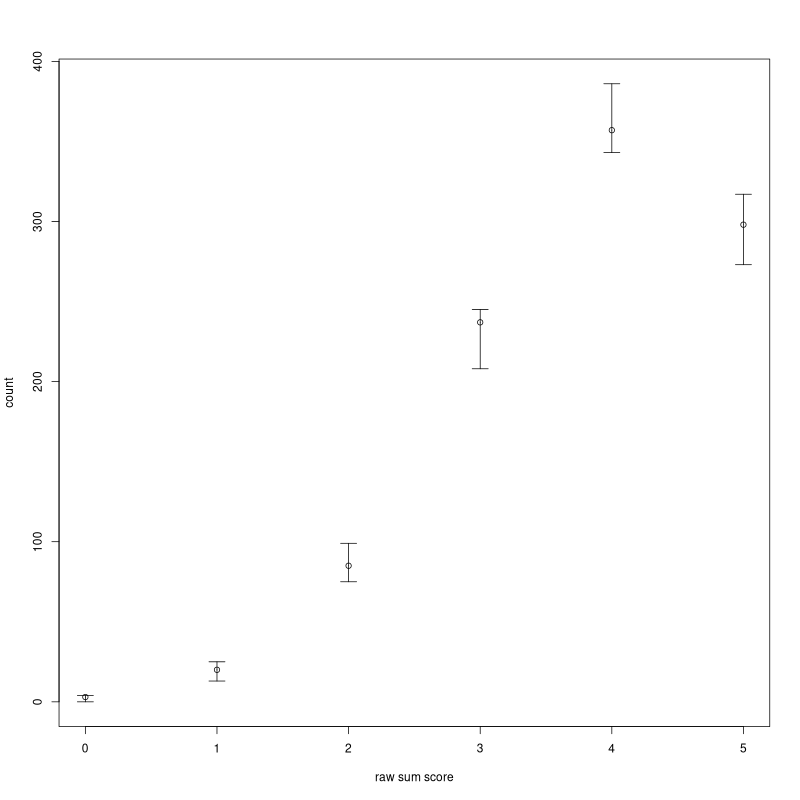
\includegraphics[scale=0.4]{Fig/raw_score_coverage.png}
  \caption{The vertical bars represent the $80\%$ HPD intervals of the predicted
  frequency distributions at each sum score, and the circles are the observed
  frequency of each sum score.}
  \label{fig:ppmc_raw_scores}
\end{figure}
The observed sum scores all fall within the $80\%$ HPD intervals of the posterior
predictive distributions. The model does seem to be able to explain the
distribution of number of correct responses well.

\subsection{Polychoric correlation coefficient}
An important assumption of the 1PNO IRT model is that discrimination parameters
across all items are equal. To check this assumption we use the polychoric
correlation coefficient. A polychoric correlation coefficient describes the
correlation between the normal variables derived from two observed ordinal
variables - in our case, the total number of correct responses of a student and
that student's item response to the $j^{th}$ item. If the model is reasonable,
then we would expect to see they polychoric correlations for all $J$ items are
similar or the variance of the polychoric correlations is close to 0. The
results in Figure~\ref{fig:ppmc_polycor}
\begin{figure}
  \centering
  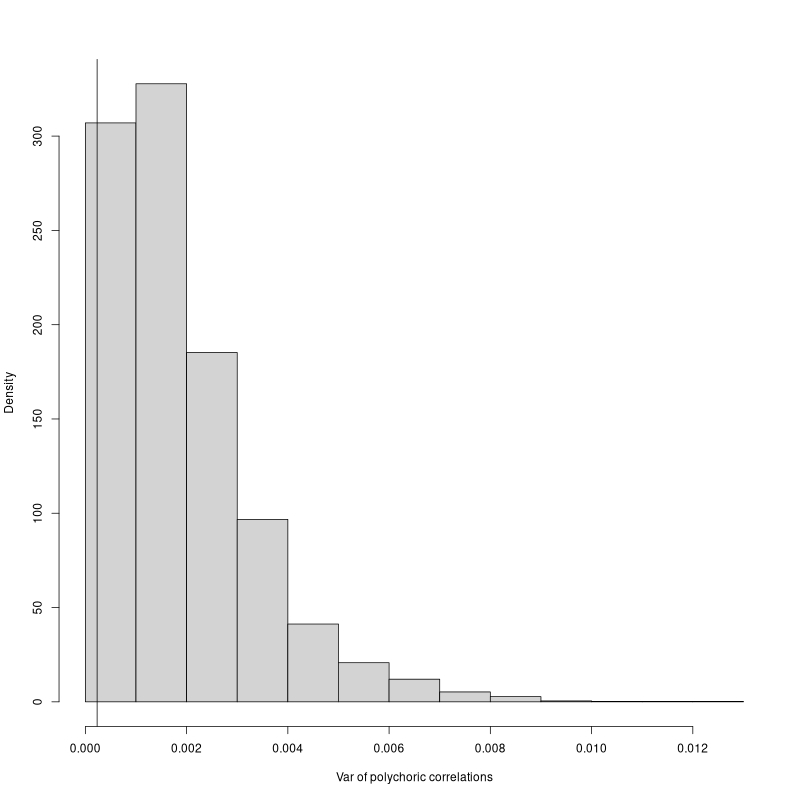
\includegraphics[scale=0.4]{Fig/ppmc_polycor.png}
  \caption{The histogram describes the posterior predictive distribution of the
  variance of the polychoric correlations of the 5 items. The vertical line is
  the observed variance of the polychoric correlations. The observed is in a
  high posterior density region.}
  \label{fig:ppmc_polycor}
\end{figure}
shows the variance of the observed polychoric correlations are very close to 0
and within a high density area of the posterior predictive distribution of the
same statistic. Consequently, there is no evidence of this aspect of misfit of
the model.

\subsection{Odds ratio}
The 1PNO IRT model assumes that item responses are independent of each other
given latent abilities $\bm{\theta}$. This is also commonly referred to as the
local independence (LI) assumption. If LI holds, the model should predict the
odds ratio of any item pairs,
\begin{equation}
  OR = \frac{n_{00} n_{11}}{n_{01} n_{10}},
\end{equation}
where $n_{kk'}$ denotes the number of students has a score $k$ on the first item
and a score $k'$ on the second item.
\begin{figure}
  \centering
  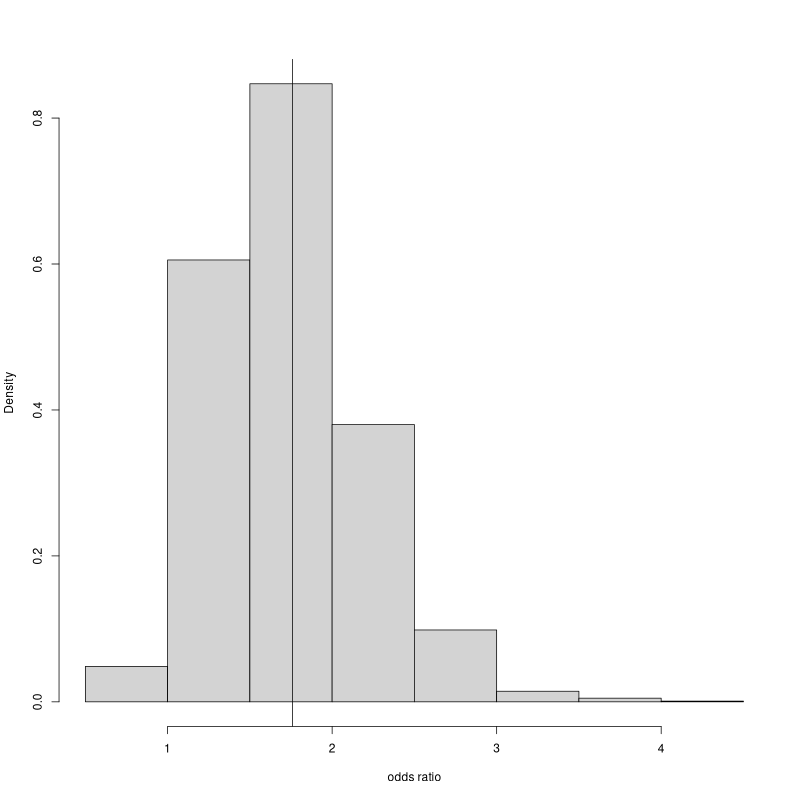
\includegraphics[scale=0.4]{Fig/ppmc_or.png}
  \caption{The histogram describes the posterior predictive distribution of the
  odds ratio of an item pair. The vertical line marks the observed odds ratio
  of that item pair.}
  \label{fig:ppmc_or}
\end{figure}
For 5 items, there are $\binom{5}{2} = 10$ pairs. For demonstration purpose, we
plot the results of one item pair in Figure~\ref{fig:ppmc_or}. The observed $OR$
is within a high density region of the posterior predictive distribution. The
examined statistic does not show evidence of violation of the LI assumption for
this pair of items.

\section{Conclusion}
In this entry, we have introduced three essential steps of the Bayesian analysis
of a psychometric model. Some more detailed concepts were demonstrated in the
context of the 1PNO IRT example. For more comprehensive review of Bayesian
methods, readers may refer to \textcite{gelman_bayesian_2013}.


\printbibliography
\end{document}
